\documentclass[twocolumn, prl]{revtex4-1}
%\usepackage{graphicx}
\usepackage[pdftex]{graphicx}
\usepackage{subfig}
\usepackage{amsmath}

\begin{document}

\newcommand{\be}{\begin{equation}}
\newcommand{\ee}{\end{equation}}


\title{Symmetry constrained machine learning}
\date{\today}

\author{Doron L. Bergman}
\affiliation{San Francisco, CA}
\email[E-mail me at: ]{doronator@gmail.com}

\begin{abstract}
Symmetry, a central concept in understanding the laws of nature, has been used for centuries in physics, mathematics, and chemistry, to help make mathematical models tractable. Yet, despite its power, symmetry has not been used extensively in machine learning, until rather recently. In this article we show a general way to incorporate symmetries into machine learning models. We demonstrate this with a detailed analysis on a rather simple real world machine learning system - a neural network for classifying handwritten digits, lacking bias terms for every neuron. We demonstrate that ignoring symmetries can have dire over-fitting consequences, and that incorporating symmetry into the model reduces over-fitting, while at the same time reducing complexity, ultimately requiring less training data, and taking less time and resources to train.
\end{abstract}

\maketitle


\section{Introduction}
\label{Sec:Intro}

% symmetry is awesome in physics!

Symmetry, together with understanding the relevant microscopic degrees of freedom and interactions, are the core ingredients behind our understanding of many body systems in the physical world.

% symmetry has not been used in ML much

In statistics and computer science, traditionally there has been little use of symmetry. The recent emergence of convolutional neural networks applied to computer vision\cite{lecun1999object, lecun1990handwritten, lecun1998gradient, krizhevsky2012imagenet, lee2009convolutional, lecun2015deep}, where translational symmetry of images is used to constrain the form of neural network models, is a first demonstration of the vast potential in building symmetries into machine learning models.

% symmetry can help in ML too!

One of the prime challenges for any sufficiently rich model is over-fitting. The physics approach to over-fitting has been to build a more constrained theory, with as few free parameters as possible. The statistics community has not had that luxury, and so they have attacked the over-fitting problem with various methods. Symmetry provides a fruitful avenue to constrain rich models, eliminating superfluous free parameters. By lowering the number of free parameters, models are not only less prone to over-fitting, they also require less data to train, and can be trained and run predictions faster.

% can we find enough symmetry in ML?

There are many obvious symmetries in vision problems - translation, rotations, and mirror images - essentially most portions of affine transformations\cite{gens2014deep, dieleman2016exploiting, cohen2016group, henriques2016warped}. Even some forms of approximate symmetry exist\cite{kiddonsymmetry} - the fact that sentences in some languages are still somewhat understandable even if the words are re-arranged, suggests natural languages have an approximate word permutation invariance. This may explain why bag of word methods are often successful, despite not retaining the full information about the word order. 
%It is the author's belief that many symmetries may be hiding in various machine learning applications, they simply need to be thought about carefully.

% Symmetry for all ... ML models
Given the benefits of combining symmetry into machine learning models, it would be useful to have a simple way to incorporate symmetries into any machine learning model. In this paper we address this problem. In short, if inputs are transformed into features that are invariant under the full symmetry group, then the model outputs will automatically be invariant as well. Are we missing any information in this way? No. Any feature that is not invariant under symmetries of the system, will spoil the model invariance, at least for some set of weights. A successful symmetry invariant feature map will be a truncated set of features that suffices to capture enough of the information to make the model successful.

% paper outline
In order to demonstrate the importance and power of symmetry invariant feature maps, we consider in this paper a very simple example - recognizing hand written digits using neural networks with bias terms absent. In section~\ref{Sec:theory}, we describe the toy model we work with to demonstrate our ideas. In section~\ref{Sec:empirics} we describe results of our empirical computer experiments confirming the mathematical theory, and demonstrating the power and ease of implementation of symmetry invariant feature maps. Finally we close with some closing remarks in section~\ref{Sec:conclusions}.


%Anecdotal evidence from the web that people use image mirroring to trick computer vision systems from identifying the content of the image:

% https://www.quora.com/Do-videos-with-reversed-image-frames-avoid-watermark-detection-by-YouTubes-copyright-identification-system

% https://www.reddit.com/r/todayilearned/comments/hqq6k/til_you_can_flipmirror_a_youtube_video_to/

\section{Theory}
\label{Sec:theory}
\subsection{Neural network model}
\label{Sec:dumb_NN}

In this section we describe the neural network model used for demonstrating the utility of symmetry invariant feature maps. The neural network model will be used on the UCI ML hand-written digits dataset available with the scikit-learn python machine learning library.

For the sake of simplicity, we will assume that our images are comprised of pixels with grayscale values scaled to the range $[-1,+1]$. We shall also use a hyperbolic tangent function as the nonlinear neuron model, rather than a logistic function, thus mapping the internal features of a neural network (NN) to the range of values $[-1, +1]$ as well. The neurons in this case are odd functions $\tanh(-x) = - \tanh(x)$. Finally, we shall not use any biases in any neuron in the system. Denoting the outputs from layer $n$ by $z^{(n)}_i$, the NN is built out of neurons performing the following function
\be
z^{(n+1)}_i = g\left(\sum_j w^n_{i, j} z^{(n)}_j\right)
\; ,
\ee
where $g(z)$ in our case is $\tanh(z)$.
The first input layer takes in the image pixels $z^0_i = x_i$. For classifying the digits, a final softmax layer produces 10 outputs which are the normalized probabilities for the image to be any one of the 10 digits
\be
p_{\alpha} = P(y=\alpha | x) \sim \exp\left[ \sum_i u_{\alpha, i} z^{(N-1)}_i \right] = {\tilde p}_{\alpha}
\ee
with the normalization
\be
p_{\alpha} = \frac{{\tilde p}_{\alpha}}{\sum_{\alpha} {\tilde p}_{\alpha} }
\; .
\ee

\subsection{Issues with symmetry}

The NN model above, with just $N=3$ layers, can achieve rather high classification accuracy of the 10 digits (see Sec.~\ref{Sec:empirics} below).
It is trained on UCI ML hand-written digits dataset available with the scikit-learn python machine learning library\cite{scikit-learn} of roughly black digits on a white background.

We note in passing that with the exception of the input layer to the neural network, at each level we can approximate a bias term, even in this architecture. In the input neuron layer, we take the sum of all the input grayscale values $\sum_i x_i$, and multiply it by a very large weight $w_0 \rightarrow \infty$. As long as the the images are majority white $\sum_i x_i > 0$, and this neuron will always output $z_0^{(1))} = g\left( w_0 \sum_i x+i \right)\approx 1$. Once there is a bias term available as an input to the second layer, another neuron in the 2nd layer can similarly approximate a bias term for the 3rd neuron layer, and so on throughout each subsequent layer $z_0^{(n+1)} = g\left( w_0 z_0^{(n)} \right)\approx 1$. This fact is probably why the neural network architecture, even without biases, is sufficiently general to train effectively on this dataset.

Next, let us challenge the system. Consider the images with the grayscale inverted, such that the digits are now roughly white on 
a black background. The inverted images still represent the same digits - the grayscale inversion transformation is therefore a symmetry of the problem. The geometric contrast is exactly the same, and so we would hope that a good machine learning system captures the geometric features of the digit themselves, and would be able to handle the inverted colors case well.

One can test this empirically (see Sec.~\ref{Sec:empirics} below), and find that the classification accuracy is quite poor, in some cases going below the accuracy of random selection (!). We explore the source of this poor performance, and prove that it is a general effect, rather than a mere anecdote.

Under the grayscale inversion symmetry, $x_i \rightarrow - x_i$, every layer except the final softmax layer is odd in its 
input. Therefore under this symmetry we get all the neuron values flipping their sign $z^{(n)}_i \rightarrow - z^{(n)}_i$. Finally, the unnormalized probabilities transform as
\be
{\tilde p}_{\alpha} \rightarrow \exp\left[ - \sum_i u_{\alpha, i} z^{(N-1)}_i \right] = 1/{\tilde p}_{\alpha}
\; .
\ee
The un-normalized probabilities are inverted. For any given image in the original dataset, the digit the model thinks has the highest probability to match the image, is also the digit with the lowest probability to match the inverted image. For every image the model identifies correctly, the inverted image gets identified incorrectly.

Let us divide the original sample set into two subsets - one for which the model correctly identifies the digit $A$, and $B$ for the remaining samples for which the model identifies the wrong digit. The accuracy rate of the model over this dataset is 
\be
R = \frac{|A|}{|A| + |B|}
\; .
\ee
All the images in $A$, when inverted, will yield the wrong digit from the model. Denoting the subset of the images for which the model identifies the digit correctly on the inverted image as ${\bar A}$, and the remaining as ${\bar B}$, we note that $A \subseteq {\bar B}$. The accuracy of the model on the inverted images is then
\be
{\bar R} = \frac{|{\bar A}|}{|{\bar A}| + |{\bar B}|} = 1 - \frac{|{\bar B}|}{|{\bar A}| + |{\bar B}|} \leq 1 - R
\; .
\ee
Written more symmetrically as $R + {\bar R} \leq 1$ this demonstrates that the accuracy over the original dataset directly constrains the accuracy that can be had on the inverted images. If the original model is accurate more than half the time over this dataset, $R>0.5$, then ${\bar R} \leq 1 - R < 0.5$. Higher accuracy on the original dataset comes directly at the expense of accuracy on the inverted images.

A model such as the one we are considering here would usually be trained on the original dataset, with only black digits on a white background. Once confronted with the reality of poor performance on the inverted images, a common approach is to simply add the additional manipulated samples to the training dataset.

However given the demonstrated $R + {\bar R} \leq 1$ constraint, if the training fully converges onto the best model, then that would suggest 
the constraint is saturated at $R + {\bar R} = 1$, and if the images and the inverted images are given equal weight in determining the model, one would expect $R = {\bar R} = 0.5$, a rather limited ceiling on the potential accuracy of the model.

This is not a very happy state of affairs. 

The weakness of this model stems from two sources - the lack of biases for each neuron, and the features we choose to work with. If we were to re-introduce the biases, what we have proved above no longer holds strictly, but since the accuracy is a smooth function of the biases, if all the biases are infinitesimally small, the upper limit on the accuracy can be only infinitesimally larger than in the vanishing biases case $R + {\bar R} \leq 1 + O(\epsilon)$.

In the next section, we consider an alternative approach, where rather than re-introducing the biases, we change the features we feed to the model. In particular, we choose features that are invariant under the inversion symmetry.

\subsection{Incorporating symmetry}
\label{Sec:symmetry_invariant_features}

What if we could construct the system to begin with to have the inversion symmetry built in to the model?
The simplest way to do this is to map the inputs (the pixels of the image) $x_i$ onto features that are invariant under the inversion symmetry.
Let us consider a generic smooth feature mapping. It can be expanded in a Taylor series
\be
f_a({\bf x}) = \sum_{n_1, n_2, \ldots} A^{(a)}_{n_1, n_2, \ldots} x_1^{n_1} x_2^{n_2} \ldots
\; .
\ee

The feature maps that are invariant under the inversion symmetry are those functions even in the inputs $x_i$ - only the even power terms are allowed
\be
f_a({\bf x}) = A^{(0)} +  \sum_{i, j} A^{(2)}_{i, j} x_i x_j + \sum_{i, j, k, \ell} A^{(4)}_{i, j, k, \ell} x_i x_j x_k x_\ell + \ldots
\; .
\ee
The lowest order feature maps that are non-trivial are the quadratic maps
\be
f_a({\bf x}) = A^{(0)} +  \sum_{i, j} A^{(2)}_{i, j} x_i x_j
\; .
\ee

If instead of the $x_i$ inputs, we fed the inversion symmetry invariant features $\chi_{i,j} = x_i x_j$ into the NN model, we would enforce the classification to be perfectly invariant under the inversion symmetry.

However, given $x_{1 \ldots M}$ pixels, the number of $\chi_{i,j}$ features is $M(M+1)/2$, a far larger number of features than the $M$ features $x_i$. Using the same neural network architecture with a much larger number of input features is not a fair comparison - there would be many more free parameters using these features than in the original model. Generally a model with more free parameters can better fit a given dataset, albeit with an increased danger of over-fitting.
To level the playing field we will choose a subset of the possible features with a similar number of free parameters
\be\label{chi_features}
\chi_i =  x_i x_{i + {\hat e}_1}
\; ,
\ee
where $i + {\hat e}_1$ denotes the pixel immediately to the right of the pixel $i$. For the edge pixels, we wrap the the index arithmetic around the boundaries of the image, essentially acting as if it were wrapped around a cylinder. The products $x_i x_{i + {\hat e}_1}$ contain information similar to a gradient of the image pixels since when both pixels are pure black or pure white, the product is +1, and when they are opposite black and white colors, it is -1. If the image were made of only extreme grayscale values - only black and white, an image made up of the $\chi_i$ features, would show the boundaries between the black and white regions of the original image.

We proceed to test the different approaches in a numerical experiment.


\section{Numerical experiment}
\label{Sec:empirics}

We use a fully connected 3-layer neural network model with 20 hidden neurons in the 1st layer, 10 in the second layer, and a softmax layer as the 3rd.
We use both a neural network with and without bias terms for comparison. We train both models on 3 separate  versions of the data - the original dataset (denoted by $X_{train}$), a combination of the original dataset, together with the inverted copy of that dataset (denoted by $\pm X_{train}$), and by the symmetry-invariant features derived from the original dataset as defined in Eq.~\eqref{chi_features} (denoted by $\chi_{train}$). We calculate the precision, recall and f1-scores on independent test datasets denoted by $X_{test}$, as well as on its inverted copy denoted by $-X_{test}$. To test the model trained on the symmetry-invariant dataset, we use yet another independent tests dataset, from which we derive the symmetry invariant features denoted $\chi_{test}$. The full results are enumerated in Table~\ref{Table:results_table}.


\begin{tabular}{ccccccc}\label{Table:results_table}
	with biases & train data & test data & accuracy & precision & recall & f1-score \\ 
	\hline
	True & $X_{train}$ & $X_{test}$ & 0.91 & 0.91 & 0.91 & 0.91 \\
	False & $X_{train}$ & $X_{test}$ & 0.89 & 0.89 & 0.89 & 0.89 \\
	%
	True & $X_{train}$ & $-X_{test}$ & $2e^{-3}$ & 0 & 0 & 0 \\
	False & $X_{train}$ & $-X_{test}$ & $1e^{-3}$ & 0 & 0 & 0 \\
	\hline
	True & $\pm X_{train}$ & $X_{test}$ & 0.88 & 0.88 & 0.88 & 0.88 \\
	False & $\pm X_{train}$ & $X_{test}$ & 0.09 & 0.08 & 0.09 & 0.06 \\
	%
	True & $\pm X_{train}$ & $-X_{test}$ & 0.82 & 0.82 & 0.81 & 0.81 \\
	False & $\pm X_{train}$ & $-X_{test}$ & 0.08 & 0.14 & 0.08 & 0.07 \\
	\hline	
	False & $\chi_{train}$ & $\chi_{test}$ & 0.89 & 0.89 & 0.89 & 0.89 \\
	\hline
\end{tabular} 


A number of findings are noteworthy. First, the $R + \bar{R} \leq 1$ limit we proved in the previous section clearly holds in our numerical experiment. Second, even a neural network model with the biases included generalizes quite poorly to the inverted samples, when trained only on the original dataset. When training on both the original dataset, and the inverted copy of it, the neural network without biases generalizes extremely poorly. The neural network with biases fairs much better. However, the neural network using the symmetry invariant features fairs best of all, though only slightly better than the neural network model with biases included trained on the original dataset and an inverted copy of it.

Our findings suggest that using symmetry invariant features may at the very least result in similar generalization quality to the standard practice of training on a transformed copy of the dataset.

\begin{figure}
\centering
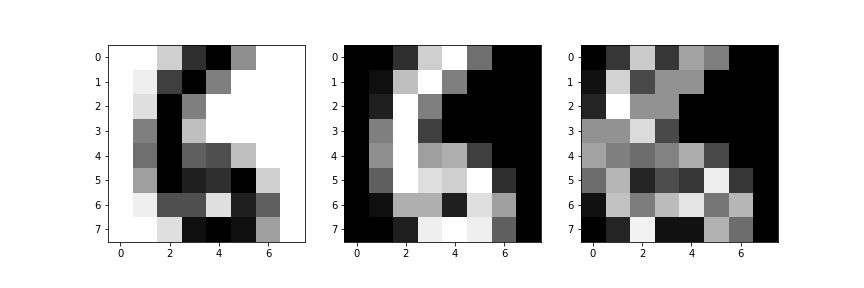
\includegraphics[width=1.0\linewidth]{images/six_cubed}
\caption{A sample image (handwritten figure 6) from the dataset (left), the image after the inversion transformation (middle), and the $\chi_i$ feature image symmetric under the inversion transformation (right).}
\label{fig:six_cubed}
\end{figure}





\section{Conclusions}
\label{Sec:conclusions}

In this article we explored the role symmetry can play in machine learning. We introduced a general way to enforce symmetry onto a machine learning model, namely to preselect features that are invariant under the symmetry transformations.

We demonstrated the dire consequences ignoring symmetry can have on the performance of a constrained family of neural network models, and how enforcing symmetry onto this model can be a benefit, and is not overly complex.

In the application of machine learning to image recognition there is a vast amount of symmetry to be found. Translational invariance, mirror reflections, at least a degree of rotational invariance, zooming in and out, as well as changing the colors themselves while maintaining contrast between different colored pixels are all transformations under which the perception of the image ought to remain unchanged. There is much more work to be done to take full advantage of these symmetries in developing more effective and robust image recognition systems.


\section{Acknowledgements}

The author would like to thank Miles Stoudenmire, Daniel Malinow, and Dmitry Novikov, for feedback on the ideas presented in this manuscript.


\vskip -0.2in

%\bibliography{A-D,E-H,I-L,M-O,P-S,T-Z}
\bibliographystyle{plainnat}
\bibliography{NN_bib}
%\bibliographystyle{TUPREP}



\vskip 0.2in

\end{document}




